\documentclass[aspectratio=169]{beamer}

\usetheme{default}
\usecolortheme{dove}

\setbeamertemplate{navigation symbols}{}
\setbeamertemplate{footline}{%
  \hfill{\large\insertframenumber\,/\,\inserttotalframenumber}\hspace{0.8em}\vspace{0.5em}%
}

\definecolor{popblue}{RGB}{52, 101, 164}
\definecolor{sampred}{RGB}{204, 0, 0}
\definecolor{paramgreen}{RGB}{0, 140, 70}
\definecolor{warnred}{RGB}{180, 40, 40}
\definecolor{orange1}{RGB}{220, 120, 0}
\definecolor{violet1}{RGB}{120, 50, 160}
\definecolor{lightbg}{RGB}{245, 245, 250}

\setbeamercolor{frametitle}{fg=popblue}
\setbeamercolor{title}{fg=popblue}

\usepackage{pgfplots}
\usepackage{tikz}
\usetikzlibrary{shapes, arrows.meta, positioning, calc, decorations.pathreplacing, patterns}
\pgfplotsset{compat=1.18}
\usepackage{amsmath, amssymb}
\usepackage{fontenc}

\title{Information Theory I: Entropy, Cross-Entropy, KL}
\subtitle{Surprisal $\cdot$ Source Coding $\cdot$ Cross-Entropy $\cdot$ KL Divergence}
\date{}

\begin{document}

% ============================================================
\begin{frame}
\titlepage
\end{frame}

% ============================================================
\begin{frame}
\frametitle{Why Information Theory?}

\begin{center}
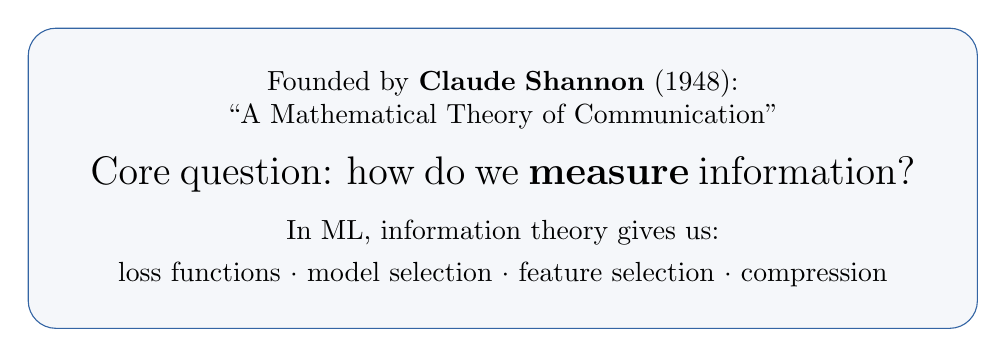
\begin{tikzpicture}
  \node[draw=popblue, fill=popblue!5, rounded corners=10pt, text width=11cm, align=center, inner sep=15pt] {
    Founded by \textbf{Claude Shannon} (1948):\\
    ``A Mathematical Theory of Communication''\\[10pt]
    {\Large Core question: how do we \textbf{measure} information?}\\[8pt]
    In ML, information theory gives us:\\[3pt]
    loss functions $\cdot$ model selection $\cdot$ feature selection $\cdot$ compression
  };
\end{tikzpicture}
\end{center}

\vspace{0.3cm}
\begin{center}
\small We'll develop three key concepts step by step:\\[4pt]
\textbf{\textcolor{paramgreen}{Entropy}} $\;\to\;$
\textbf{\textcolor{orange1}{Cross-Entropy}} $\;\to\;$
\textbf{\textcolor{sampred}{KL Divergence}}
\end{center}
\end{frame}

% ============================================================
\section{Entropy}

\begin{frame}
\begin{center}
\vspace{1cm}
{\LARGE\bfseries\textcolor{popblue}{Entropy}}\\[15pt]
{\large How much \textbf{surprise} does a random variable carry?}\\[4pt]
{\large Can we quantify \textbf{uncertainty}?}
\end{center}
\end{frame}

% ============================================================
\begin{frame}
\frametitle{Surprisal: Rare Events Are More Informative}

\small
Observing a \textbf{rare} event is more ``surprising'' than observing a common one.

\vspace{0.1cm}
\begin{center}
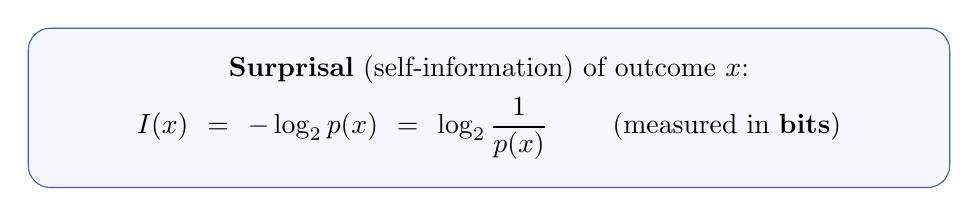
\begin{tikzpicture}
  \node[draw=popblue, fill=popblue!5, rounded corners=8pt, text width=11cm, align=center, inner sep=10pt] {
    \textbf{Surprisal} (self-information) of outcome $x$:\\[4pt]
    $I(x) = -\log_2 p(x) = \log_2 \dfrac{1}{p(x)}$ \qquad(measured in \textbf{bits})
  };
\end{tikzpicture}
\end{center}

\vspace{-0.1cm}
\begin{columns}[T]
\begin{column}{0.48\textwidth}
\begin{center}
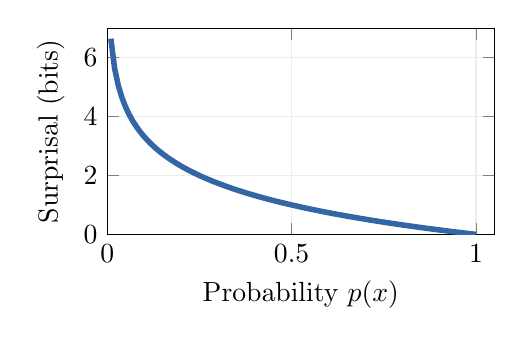
\begin{tikzpicture}
  \begin{axis}[
    width=6.5cm, height=4.2cm,
    xlabel={Probability $p(x)$},
    ylabel={Surprisal (bits)},
    domain=0.01:1,
    xmin=0, xmax=1.05,
    ymin=0, ymax=7,
    grid=major, grid style={gray!15},
    every axis plot/.append style={line width=2pt},
  ]
    \addplot[popblue, samples=100] {-ln(x)/ln(2)};
  \end{axis}
\end{tikzpicture}
\end{center}
\end{column}
\begin{column}{0.48\textwidth}
\vspace{0.2cm}
\textbf{Properties:}
\begin{itemize}\setlength{\itemsep}{3pt}
  \item $I(x) \geq 0$ always
  \item $p(x) = 1 \;\Rightarrow\; I(x) = 0$ (certain $=$ no surprise)
  \item $p(x) \to 0 \;\Rightarrow\; I(x) \to \infty$ (rare $=$ very surprising)
  \item \textbf{Additive:} $I(x,y) = I(x) + I(y)$ for independent events
\end{itemize}
\end{column}
\end{columns}
\end{frame}

% ============================================================
\begin{frame}
\frametitle{Shannon Entropy = Expected Surprisal}

\small
We can't predict which outcome we'll see, so we take the \textbf{average} surprisal:

\vspace{0.1cm}
\begin{center}
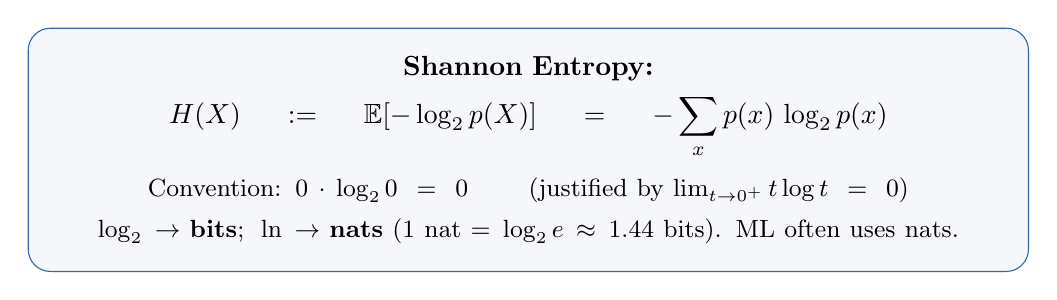
\begin{tikzpicture}
  \node[draw=popblue, fill=popblue!5, rounded corners=8pt, text width=12cm, align=center, inner sep=10pt] {
    \textbf{Shannon Entropy:}\\[4pt]
    $H(X) \;:=\; \mathbb{E}\!\left[-\log_2 p(X)\right] \;=\; -\displaystyle\sum_{x} p(x)\,\log_2 p(x)$\\[6pt]
    \small Convention: $0 \cdot \log_2 0 = 0$ \qquad(justified by $\lim_{t\to 0^+} t\log t = 0$)\\[3pt]
    \small $\log_2 \to$ \textbf{bits}; \;$\ln \to$ \textbf{nats} (1 nat $= \log_2 e \approx 1.44$ bits). ML often uses nats.
  };
\end{tikzpicture}
\end{center}

\vspace{0.1cm}
\textbf{Worked example:} $X$ takes values $\{a, b, c, d\}$ with $p = \left(\frac{1}{2},\; \frac{1}{4},\; \frac{1}{8},\; \frac{1}{8}\right)$.

\vspace{-0.1cm}
\begin{align*}
  H(X) &= -\left[\tfrac{1}{2}\log_2\tfrac{1}{2} + \tfrac{1}{4}\log_2\tfrac{1}{4} + \tfrac{1}{8}\log_2\tfrac{1}{8} + \tfrac{1}{8}\log_2\tfrac{1}{8}\right]\\
  &= \tfrac{1}{2}\cdot 1 + \tfrac{1}{4}\cdot 2 + \tfrac{1}{8}\cdot 3 + \tfrac{1}{8}\cdot 3 = \boxed{\tfrac{7}{4} = 1.75 \;\text{bits}}
\end{align*}
\end{frame}

% ============================================================
\begin{frame}
\frametitle{Entropy of the Bernoulli Distribution}

For $X \sim \text{Bern}(s)$: \;$P(X{=}1) = s$, \;$P(X{=}0) = 1-s$.

$$H(X) = -s\log_2 s - (1-s)\log_2(1-s)$$

\begin{center}
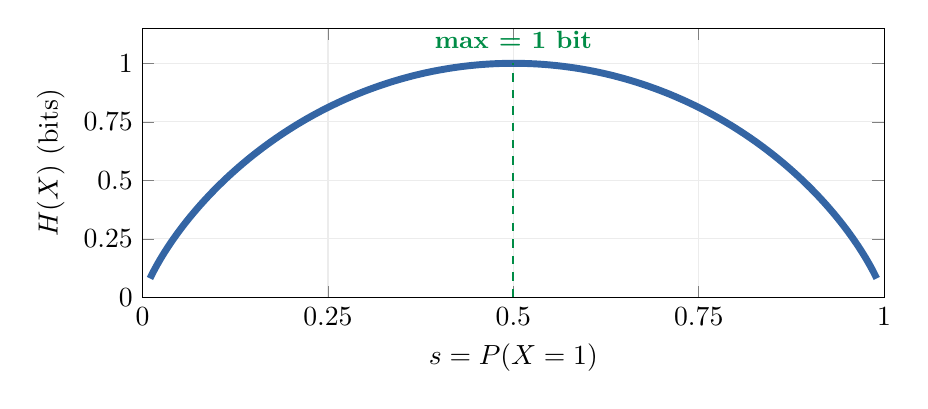
\begin{tikzpicture}
  \begin{axis}[
    width=11cm, height=5cm,
    xlabel={$s = P(X=1)$},
    ylabel={$H(X)$ (bits)},
    domain=0.01:0.99,
    xmin=0, xmax=1,
    ymin=0, ymax=1.15,
    grid=major, grid style={gray!15},
    xtick={0, 0.25, 0.5, 0.75, 1},
    ytick={0, 0.25, 0.5, 0.75, 1},
    every axis plot/.append style={line width=2.5pt},
  ]
    \addplot[popblue, samples=200] {-x*ln(x)/ln(2) - (1-x)*ln(1-x)/ln(2)};
    \draw[dashed, thick, paramgreen] (axis cs:0.5, 0) -- (axis cs:0.5, 1);
    \node[font=\small\bfseries, paramgreen] at (axis cs:0.5, 1.1) {max = 1 bit};
  \end{axis}
\end{tikzpicture}
\end{center}

\vspace{-0.2cm}
\begin{center}
\small $H(0) = H(1) = 0$ (deterministic). \quad $H(0.5) = 1$ bit (fair coin: maximum uncertainty).
\end{center}
\end{frame}

% ============================================================
\begin{frame}
\frametitle{Properties of Entropy}

\renewcommand{\arraystretch}{1.5}
\begin{center}
\begin{tabular}{clc}
  \textbf{\#} & \textbf{Property} & \textbf{Formula} \\
  \hline
  1 & \textbf{Non-negative} & $H(X) \geq 0$ \\
  2 & \textbf{Zero for deterministic} & $H(X) = 0$ iff one $p(x) = 1$ \\
  3 & \textbf{Continuous} in probabilities & small $\Delta p \Rightarrow$ small $\Delta H$ \\
  4 & \textbf{Symmetric} in $p$ values & relabeling outcomes doesn't change $H$ \\
  5 & \textbf{Additive} for independent RVs & $H(X,Y) = H(X) + H(Y)$ \\
  6 & \textbf{Maximal for uniform} & $H(X) \leq \log_2 g$ \;($g$ = \#outcomes) \\
  \hline
\end{tabular}
\end{center}

\vspace{0.1cm}
\begin{center}
\fcolorbox{orange1}{orange1!5}{\parbox{11cm}{\centering\small
  \textbf{Uniqueness (Khinchin, 1957):} Shannon entropy is the \textbf{only} function
  satisfying properties 1--5 (up to a constant). There is no other sensible measure of uncertainty!
}}
\end{center}
\end{frame}

% ============================================================
\begin{frame}
\frametitle{Entropy Is Maximal for Uniform Distributions}

\small
\textbf{Claim:} Among all distributions on $g$ outcomes, the uniform maximizes entropy.

\vspace{0.15cm}
\textbf{Proof} (Lagrange multipliers): Maximize $H = -\sum_{i=1}^g p_i \log_2 p_i$ subject to $\sum p_i = 1$.

\vspace{-0.1cm}
$$\mathcal{L} = -\sum_{i=1}^g p_i \log_2 p_i \;-\; \lambda\!\left(\sum_{i=1}^g p_i - 1\right)$$

\pause
$$\frac{\partial \mathcal{L}}{\partial p_i} = -\log_2 p_i - \frac{1}{\ln 2} - \lambda = 0
\quad\Rightarrow\quad \log_2 p_i = \text{const}
\quad\Rightarrow\quad \boxed{p_i = \frac{1}{g} \;\;\text{for all } i}$$

\vspace{0.1cm}
$$H_{\max} = -\sum_{i=1}^g \frac{1}{g}\log_2\frac{1}{g} = \log_2 g$$

\vspace{0.1cm}
\begin{center}
\fcolorbox{paramgreen}{paramgreen!5}{\parbox{11cm}{\centering\small
  \textbf{Intuition:} The uniform distribution is the ``most uncertain'' ---
  it makes no assumptions about which outcome is more likely.\\[3pt]
  More outcomes $\Rightarrow$ higher maximum entropy, but with diminishing returns.
}}
\end{center}
\end{frame}

% ============================================================
\section{Source Coding}

\begin{frame}
\begin{center}
\vspace{1cm}
{\LARGE\bfseries\textcolor{popblue}{Source Coding}}\\[15pt]
{\large Entropy measures uncertainty. But what IS information, \textbf{physically}?}\\[4pt]
{\large Source coding gives a concrete answer: \textbf{bits}.}
\end{center}
\end{frame}

% ============================================================
\begin{frame}
\frametitle{The Coding Problem}

\small
A source produces symbols from $\mathcal{X} = \{\text{dog, cat, fish, bird}\}$.
We want to encode them as \textbf{binary strings} for transmission.

\vspace{0.2cm}
\textbf{Fixed-length code:} Each symbol gets a codeword of the same length.

\vspace{0.1cm}
\begin{center}
\renewcommand{\arraystretch}{1.4}
\begin{tabular}{lccl}
  \textbf{Symbol} & \textbf{Probability} & \textbf{Codeword} & \textbf{Length} \\
  \hline
  dog  & $1/2$ & 00 & 2 bits \\
  cat  & $1/4$ & 01 & 2 bits \\
  fish & $1/8$ & 10 & 2 bits \\
  bird & $1/8$ & 11 & 2 bits \\
  \hline
\end{tabular}
\end{center}

$$\mathbb{E}[L] = \tfrac{1}{2}\cdot 2 + \tfrac{1}{4}\cdot 2 + \tfrac{1}{8}\cdot 2 + \tfrac{1}{8}\cdot 2 = \textbf{2 bits per symbol}$$

\vspace{0.05cm}
\begin{center}
\small But ``dog'' appears \textbf{half} the time --- shouldn't it get a \textbf{shorter} code?
\end{center}
\end{frame}

% ============================================================
\begin{frame}
\frametitle{Variable-Length Codes and the Prefix Property}

\small
\textbf{Idea:} Shorter codes for more probable symbols, longer for less probable.

\vspace{0.1cm}
\textbf{Problem:} Ambiguity!  If dog$\to$\texttt{0}, cat$\to$\texttt{1}, fish$\to$\texttt{01}, bird$\to$\texttt{11},
then \texttt{01} could be ``dog, cat'' or ``fish'' --- we can't tell!

\vspace{0.1cm}
\begin{center}
\fcolorbox{popblue}{popblue!5}{\parbox{11cm}{\centering\small
  \textbf{Prefix property:} No codeword is a prefix of another codeword.\\[2pt]
  Guarantees \textbf{unambiguous decoding} --- read left-to-right, always know where each codeword ends.
}}
\end{center}

\vspace{0.05cm}
\textbf{Solution --- a valid prefix code:}
\vspace{-0.1cm}
\begin{center}
\renewcommand{\arraystretch}{1.2}
\begin{tabular}{lcccc}
  \textbf{Symbol} & \textbf{Prob.}~$p(x)$ & \textbf{Codeword} & \textbf{Length} $L(x)$ & \textbf{Surprisal} $-\log_2 p(x)$ \\
  \hline
  dog  & $1/2$ & \texttt{0}   & 1 & 1 \\
  cat  & $1/4$ & \texttt{10}  & 2 & 2 \\
  fish & $1/8$ & \texttt{110} & 3 & 3 \\
  bird & $1/8$ & \texttt{111} & 3 & 3 \\
  \hline
\end{tabular}
\end{center}
\end{frame}

% ============================================================
\begin{frame}
\frametitle{Prefix Code as a Binary Tree}

\begin{center}
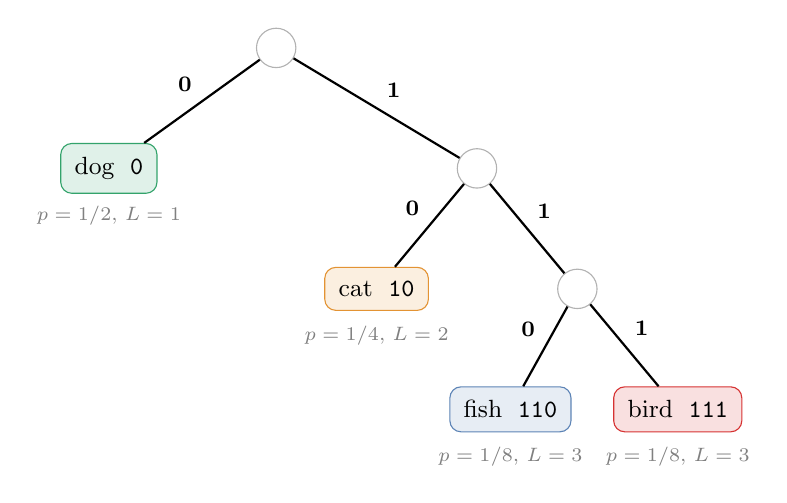
\begin{tikzpicture}[scale=0.85,
  nd/.style={circle, draw=gray!60, fill=white, minimum size=5mm, inner sep=0pt},
  lf/.style={rounded corners=4pt, draw=#1!80, fill=#1!12, font=\small, inner sep=5pt},
]
  % Nodes
  \node[nd] (r) at (0,0) {};
  \node[nd] (n1) at (3,-1.8) {};
  \node[nd] (n2) at (4.5,-3.6) {};
  % Leaves
  \node[lf=paramgreen] (dog)  at (-2.5,-1.8) {dog \;\texttt{0}};
  \node[lf=orange1]    (cat)  at (1.5,-3.6)  {cat \;\texttt{10}};
  \node[lf=popblue]    (fish) at (3.5,-5.4)  {fish \;\texttt{110}};
  \node[lf=sampred]    (bird) at (6,-5.4)    {bird \;\texttt{111}};
  % Edges
  \draw[thick] (r) -- node[above left, font=\footnotesize\bfseries] {0} (dog);
  \draw[thick] (r) -- node[above right, font=\footnotesize\bfseries] {1} (n1);
  \draw[thick] (n1) -- node[above left, font=\footnotesize\bfseries] {0} (cat);
  \draw[thick] (n1) -- node[above right, font=\footnotesize\bfseries] {1} (n2);
  \draw[thick] (n2) -- node[above left, font=\footnotesize\bfseries] {0} (fish);
  \draw[thick] (n2) -- node[above right, font=\footnotesize\bfseries] {1} (bird);
  % Probabilities
  \node[font=\scriptsize, gray] at (-2.5,-2.5) {$p = 1/2$, $L = 1$};
  \node[font=\scriptsize, gray] at (1.5,-4.3)  {$p = 1/4$, $L = 2$};
  \node[font=\scriptsize, gray] at (3.5,-6.1)  {$p = 1/8$, $L = 3$};
  \node[font=\scriptsize, gray] at (6,-6.1)    {$p = 1/8$, $L = 3$};
\end{tikzpicture}
\end{center}

\vspace{-0.1cm}
\begin{center}
\small Shorter paths (fewer bits) for more probable symbols.\\
Each leaf is a codeword; the prefix property is guaranteed by the tree structure.
\end{center}
\end{frame}

% ============================================================
\begin{frame}
\frametitle{Optimal Code Length Equals Entropy}

\small
\textbf{Key observation:} In our prefix code, the code length of each symbol equals its surprisal!

$$L(x) = -\log_2 p(x) \qquad\text{for every symbol } x$$

\pause
\vspace{0.1cm}
The \textbf{expected code length}:
\begin{align*}
  \mathbb{E}[L(X)] &= \sum_x p(x)\,L(x) = \sum_x p(x)\cdot\bigl(-\log_2 p(x)\bigr)\\[4pt]
  &= \tfrac{1}{2}\cdot 1 + \tfrac{1}{4}\cdot 2 + \tfrac{1}{8}\cdot 3 + \tfrac{1}{8}\cdot 3 = \textbf{1.75 bits}\\[4pt]
  &= H(X) \quad\textcolor{paramgreen}{\checkmark}
\end{align*}

\vspace{0.1cm}
\begin{center}
\fcolorbox{paramgreen}{paramgreen!5}{\parbox{11cm}{\centering
  The optimal prefix code assigns $-\log_2 p(x)$ bits to symbol $x$.\\[3pt]
  The \textbf{average code length} of this optimal code is exactly \textbf{the entropy} $H(X)$.\\[3pt]
  \small Compared to fixed-length (2 bits): we save $2 - 1.75 = 0.25$ bits per symbol!
}}
\end{center}
\end{frame}

% ============================================================
\begin{frame}
\frametitle{Shannon's Source Coding Theorem}

\begin{center}
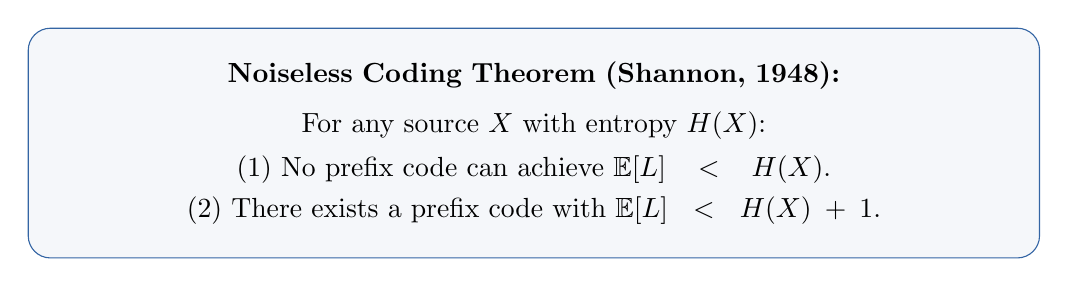
\begin{tikzpicture}
  \node[draw=popblue, fill=popblue!5, rounded corners=8pt, text width=12cm, align=center, inner sep=12pt] {
    \textbf{Noiseless Coding Theorem (Shannon, 1948):}\\[6pt]
    For any source $X$ with entropy $H(X)$:\\[4pt]
    (1) No prefix code can achieve $\mathbb{E}[L] < H(X)$.\\[3pt]
    (2) There exists a prefix code with $\mathbb{E}[L] < H(X) + 1$.
  };
\end{tikzpicture}
\end{center}

\vspace{0.3cm}
\begin{center}
\fcolorbox{orange1}{orange1!5}{\parbox{11cm}{\centering\small
  \textbf{Entropy = the fundamental limit of lossless compression.}\\[3pt]
  If you try to use fewer bits on average, you \textbf{must} lose information.\\[3pt]
  In practice: \textbf{Huffman coding} achieves near-optimal code lengths.
}}
\end{center}

\vspace{0.2cm}
\begin{center}
\small\textbf{This gives entropy a physical meaning:} $H(X)$ = minimum average bits needed to describe $X$.
\end{center}
\end{frame}

% ============================================================
\section{Cross-Entropy}

\begin{frame}
\begin{center}
\vspace{1cm}
{\LARGE\bfseries\textcolor{popblue}{Cross-Entropy}}\\[15pt]
{\large What happens when we use the \textbf{wrong} code?}
\end{center}
\end{frame}

% ============================================================
\begin{frame}
\frametitle{Using the Wrong Codebook}

\small
The true distribution is $p$, but we \textbf{think} the distribution is $q$ (and design our code for $q$).

\vspace{0.15cm}
\begin{center}
\renewcommand{\arraystretch}{1.4}
\begin{tabular}{lccccc}
  \textbf{Symbol} & $p(x)$ & $q(x)$ & $L_p(x) = -\log_2 p$ & $L_q(x) = -\log_2 q$ & \textbf{Waste} \\
  \hline
  dog  & $1/2$ & $1/4$ & 1 & 2 & \textcolor{sampred}{+1} \\
  cat  & $1/4$ & $1/4$ & 2 & 2 & 0 \\
  fish & $1/8$ & $1/4$ & 3 & 2 & \textcolor{paramgreen}{$-$1} \\
  bird & $1/8$ & $1/4$ & 3 & 2 & \textcolor{paramgreen}{$-$1} \\
  \hline
\end{tabular}
\end{center}

\vspace{0.1cm}
Expected length with the \textbf{right} code (for $p$): $\;\mathbb{E}_p[L_p] = H(p) = 1.75$ bits.\\
Expected length with the \textbf{wrong} code (for $q$): $\;\mathbb{E}_p[L_q] = \tfrac{1}{2}\cdot 2 + \tfrac{1}{4}\cdot 2 + \tfrac{1}{8}\cdot 2 + \tfrac{1}{8}\cdot 2 = 2$ bits.

\vspace{0.15cm}
\begin{center}
\fcolorbox{sampred}{sampred!5}{\parbox{11cm}{\centering\small
  Using the wrong code wastes $2 - 1.75 = 0.25$ bits per symbol on average.\\
  The wrong code is \textbf{always at least as long} as the right one.
}}
\end{center}
\end{frame}

% ============================================================
\begin{frame}
\frametitle{Cross-Entropy: Definition}

\begin{center}
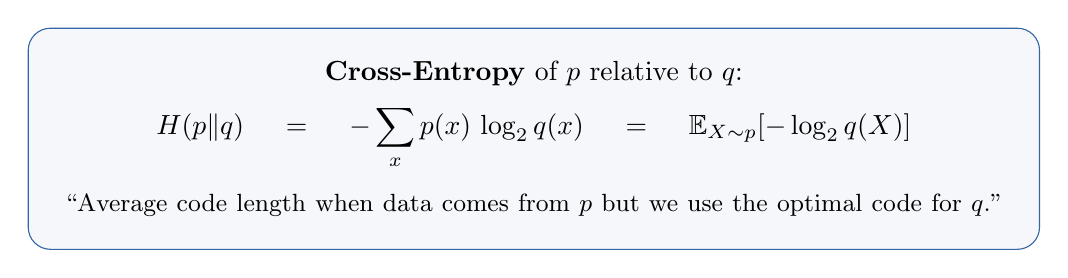
\begin{tikzpicture}
  \node[draw=popblue, fill=popblue!5, rounded corners=8pt, text width=12cm, align=center, inner sep=12pt] {
    \textbf{Cross-Entropy} of $p$ relative to $q$:\\[6pt]
    $H(p \| q) \;=\; -\displaystyle\sum_{x} p(x)\,\log_2 q(x) \;=\; \mathbb{E}_{X \sim p}\!\left[-\log_2 q(X)\right]$\\[8pt]
    \small ``Average code length when data comes from $p$ but we use the optimal code for $q$.''
  };
\end{tikzpicture}
\end{center}

\vspace{0.3cm}
\begin{center}
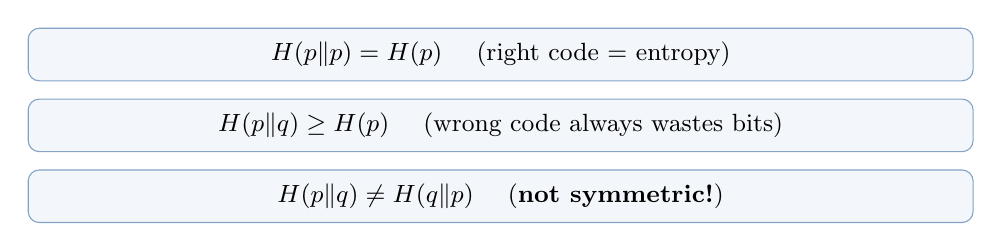
\begin{tikzpicture}[
  pbox/.style={draw=popblue!60, fill=popblue!6, rounded corners=4pt, minimum width=12cm, align=center, font=\small, inner sep=5pt}
]
  \node[pbox] at (0, 0.8) {$H(p \| p) = H(p)$ \quad(right code $=$ entropy)};
  \node[pbox] at (0, -0.1) {$H(p \| q) \geq H(p)$ \quad(wrong code always wastes bits)};
  \node[pbox] at (0, -1.0) {$H(p \| q) \neq H(q \| p)$ \quad(\textbf{not symmetric!})};
\end{tikzpicture}
\end{center}
\end{frame}

% ============================================================
\section{KL Divergence}

\begin{frame}
\begin{center}
\vspace{1cm}
{\LARGE\bfseries\textcolor{popblue}{KL Divergence}}\\[15pt]
{\large How many bits do we \textbf{waste} by using the wrong code?}
\end{center}
\end{frame}

% ============================================================
\begin{frame}
\frametitle{From Cross-Entropy to KL Divergence}

\small
The \textbf{gap} between cross-entropy and entropy measures the wasted bits:

\vspace{-0.2cm}
\begin{align*}
  \underbrace{H(p \| q)}_{\text{wrong code}} - \underbrace{H(p)}_{\text{right code}}
  &= -\sum_x p(x)\log_2 q(x) - \left(-\sum_x p(x)\log_2 p(x)\right)\\[2pt]
  &= \sum_x p(x)\left[\log_2 p(x) - \log_2 q(x)\right]\\[2pt]
  &= \sum_x p(x)\,\log_2 \frac{p(x)}{q(x)}
\end{align*}

\pause
\vspace{-0.35cm}
\begin{center}
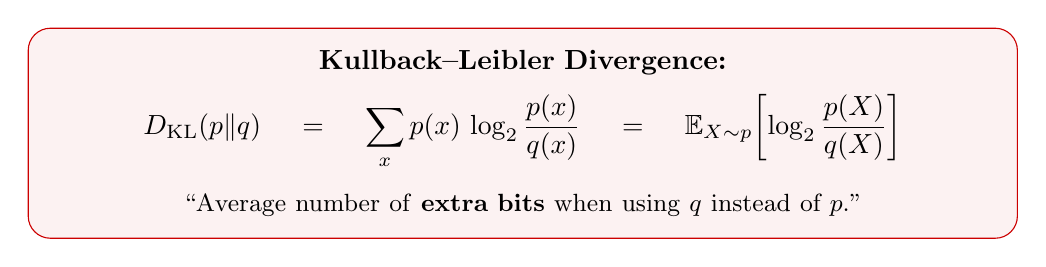
\begin{tikzpicture}
  \node[draw=sampred, fill=sampred!5, rounded corners=8pt, text width=12cm, align=center, inner sep=8pt] {
    \textbf{Kullback--Leibler Divergence:}\\[6pt]
    $D_{\text{KL}}(p \| q) \;=\; \displaystyle\sum_{x} p(x)\,\log_2\frac{p(x)}{q(x)} \;=\; \mathbb{E}_{X \sim p}\!\left[\log_2\frac{p(X)}{q(X)}\right]$\\[8pt]
    \small ``Average number of \textbf{extra bits} when using $q$ instead of $p$.''
  };
\end{tikzpicture}
\end{center}
\end{frame}

% ============================================================
\begin{frame}
\frametitle{The Fundamental Identity}

\vspace{0.3cm}
\begin{center}
$$\boxed{H(p \| q) \;=\; H(p) \;+\; D_{\text{KL}}(p \| q)}$$
\end{center}

\vspace{0.2cm}
\begin{center}
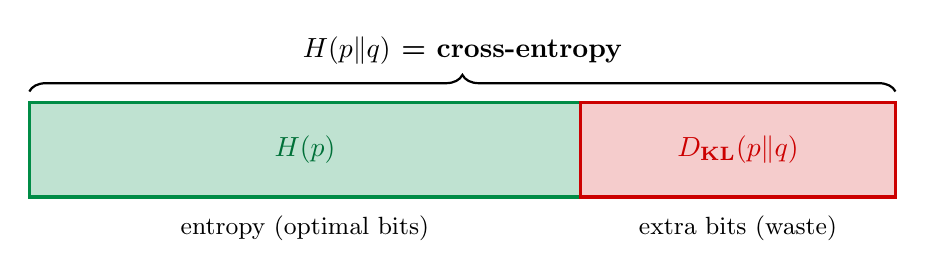
\begin{tikzpicture}
  % Full bar: cross-entropy
  \fill[popblue!15] (0,0) rectangle (11, 1.2);
  \draw[very thick, popblue] (0,0) rectangle (11, 1.2);

  % Entropy portion
  \fill[paramgreen!25] (0,0) rectangle (7, 1.2);
  \draw[very thick, paramgreen] (0,0) rectangle (7, 1.2);
  \node[font=\normalsize\bfseries, paramgreen!80!black] at (3.5, 0.6) {$H(p)$};

  % KL portion
  \fill[sampred!20] (7,0) rectangle (11, 1.2);
  \draw[very thick, sampred] (7,0) rectangle (11, 1.2);
  \node[font=\normalsize\bfseries, sampred] at (9, 0.6) {$D_{\text{KL}}(p \| q)$};

  % Labels below
  \node[font=\small] at (3.5, -0.4) {entropy (optimal bits)};
  \node[font=\small] at (9, -0.4) {extra bits (waste)};

  % Brace on top
  \draw[decorate, decoration={brace, amplitude=6pt, raise=4pt}, thick]
    (0, 1.2) -- (11, 1.2) node[midway, above, yshift=10pt, font=\normalsize\bfseries] {$H(p \| q)$ = cross-entropy};
\end{tikzpicture}
\end{center}

\vspace{0.2cm}
\begin{center}
\fcolorbox{orange1}{orange1!5}{\parbox{11cm}{\centering\small
  Since $D_{\text{KL}}(p \| q) \geq 0$ (we'll prove this next), cross-entropy \textbf{always}
  exceeds entropy:\\[2pt]
  $H(p \| q) \geq H(p)$, with equality iff $p = q$.
}}
\end{center}
\end{frame}

% ============================================================
\begin{frame}
\frametitle{Information Inequality: $D_{\text{KL}} \geq 0$}

\small
\textbf{Gibbs' Inequality:} $D_{\text{KL}}(p \| q) \geq 0$, with equality iff $p = q$.

\vspace{0.05cm}
\textbf{Proof} (via Jensen's inequality, since $\log$ is concave):

\vspace{-0.25cm}
\begin{align*}
  -D_{\text{KL}}(p \| q) &= \sum_x p(x)\,\log\frac{q(x)}{p(x)} &\text{(flip the ratio)}\\[2pt]
  &\leq \log\!\left(\sum_x p(x)\cdot\frac{q(x)}{p(x)}\right) &\text{(Jensen: $\mathbb{E}[\log Z] \leq \log\mathbb{E}[Z]$)}\\[2pt]
  &= \log\!\left(\sum_x q(x)\right) = \log 1 = 0
\end{align*}

\vspace{-0.4cm}
$$\Rightarrow\quad D_{\text{KL}}(p \| q) \geq 0$$

\vspace{-0.4cm}\pause
Equality iff $q(x)/p(x)$ is constant $\forall\, x$ (strict concavity of $\log$), i.e., $p = q$.

\vspace{0.05cm}
\begin{center}
\fcolorbox{paramgreen}{paramgreen!5}{\parbox{10.5cm}{\centering\small
  \textbf{The most fundamental inequality in information theory.}\\[2pt]
  You can never do better than the optimal code. Using any other distribution wastes bits.
}}
\end{center}
\end{frame}

% ============================================================
\begin{frame}
\frametitle{KL Divergence Is Not a Distance}

\small
Despite measuring ``closeness,'' $D_{\text{KL}}$ is \textbf{not a distance}:

\vspace{0.2cm}
\begin{center}
\renewcommand{\arraystretch}{1.6}
\begin{tabular}{lcc}
  \textbf{Property} & \textbf{True distance?} & \textbf{KL?} \\
  \hline
  Non-negativity: $d(p,q) \geq 0$ & \textcolor{paramgreen}{\checkmark} & \textcolor{paramgreen}{\checkmark} \\
  Identity: $d(p,q) = 0 \Leftrightarrow p = q$ & \textcolor{paramgreen}{\checkmark} & \textcolor{paramgreen}{\checkmark} \\
  Symmetry: $d(p,q) = d(q,p)$ & \textcolor{paramgreen}{\checkmark} & \textcolor{sampred}{\textbf{$\times$}} \\
  Triangle inequality & \textcolor{paramgreen}{\checkmark} & \textcolor{sampred}{\textbf{$\times$}} \\
  \hline
\end{tabular}
\end{center}

\vspace{0.2cm}
\textbf{Example:} $p = \text{Bern}(0.1)$, $q = \text{Bern}(0.5)$.

\vspace{0.1cm}
\begin{center}

\begin{tikzpicture}[
  pbox/.style={draw=popblue!60, fill=popblue!6, rounded corners=4pt, minimum width=6cm, align=center, font=\small, inner sep=5pt}
]
  \node[pbox] at (-3.5, 0) {$D_{\text{KL}}(p \| q) \approx 0.53$ bits};
  \node[pbox] at (3.5, 0)  {$D_{\text{KL}}(q \| p) \approx 0.74$ bits};
  \node[font=\Large\bfseries, sampred] at (0, 0) {$\neq$};
\end{tikzpicture}
\end{center}

\vspace{0.1cm}
\begin{center}
\small KL is a \textbf{divergence}, not a distance. The asymmetry will matter a lot in ML!
\end{center}
\end{frame}

% ============================================================
\begin{frame}
\frametitle{Three Interpretations of KL Divergence}

\begin{center}
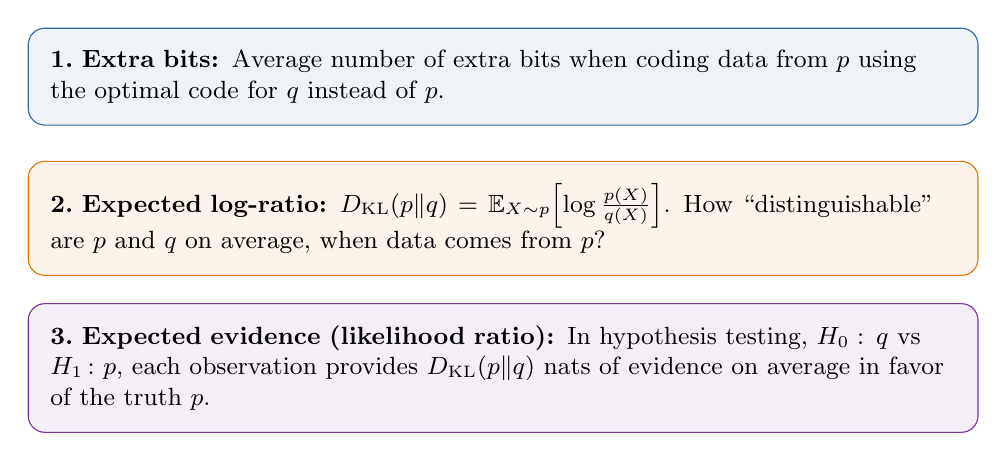
\begin{tikzpicture}[
  box/.style={draw=#1, fill=#1!8, rounded corners=6pt, text width=11.5cm, align=left, inner sep=8pt, font=\small},
]
  \node[box=popblue] at (0, 2.3) {
    \textbf{1.~Extra bits:} Average number of extra bits when coding data from $p$
    using the optimal code for $q$ instead of $p$.
  };
  \node[box=orange1] at (0, 0.5) {
    \textbf{2.~Expected log-ratio:} $D_{\text{KL}}(p \| q) = \mathbb{E}_{X \sim p}\!\left[\log\frac{p(X)}{q(X)}\right]$.
    How ``distinguishable'' are $p$ and $q$ on average, when data comes from $p$?
  };
  \node[box=violet1] at (0, -1.4) {
    \textbf{3.~Expected evidence (likelihood ratio):} In hypothesis testing,
    $H_0\!: q$ vs $H_1\!: p$, each observation provides
    $D_{\text{KL}}(p \| q)$ nats of evidence on average in favor of the truth $p$.
  };
\end{tikzpicture}
\end{center}

\vspace{0.1cm}
\begin{center}
\small All three interpretations say the same thing:
$D_{\text{KL}}$ measures \textbf{how different $q$ is from $p$, as seen by $p$}.
\end{center}
\end{frame}

% ============================================================
\begin{frame}
\frametitle{Differential Entropy (Brief)}

\small
For \textbf{continuous} RVs with density $f(x)$, entropy generalizes to:

$$h(X) = -\int f(x)\,\log f(x)\,dx$$

\vspace{-0.1cm}
\begin{center}
\renewcommand{\arraystretch}{1.6}
\begin{tabular}{lcc}
  \textbf{Distribution} & \textbf{Differential entropy} $h(X)$ & \textbf{Depends on} \\
  \hline
  $\text{Uniform}[0, a]$ & $\log a$ & support width \\
  $N(\mu, \sigma^2)$ & $\frac{1}{2}\log(2\pi e\,\sigma^2)$ & variance only \\
  \hline
\end{tabular}
\end{center}

\vspace{0.1cm}
\begin{center}
\fcolorbox{warnred}{warnred!5}{\parbox{11cm}{\centering\small
  \textbf{Warning:} Differential entropy can be \textbf{negative}!\\
  E.g., $\text{Uniform}[0, 1/2]$: $h(X) = \log(1/2) = -1$ bit.\\[3pt]
  It is \textbf{not} invariant to coordinate changes. Use with care.\\[3pt]
  The KL divergence $D_{\text{KL}}(p \| q) = \int p\log\frac{p}{q}$ remains well-behaved for continuous distributions.
}}
\end{center}
\end{frame}

% ============================================================
\section{Summary}

\begin{frame}
\frametitle{The Big Picture}

\begin{center}
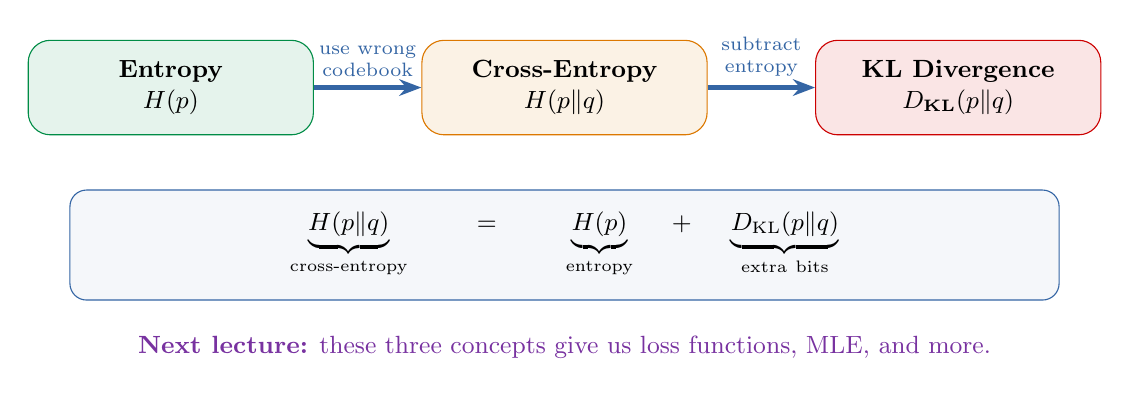
\begin{tikzpicture}[
  concept/.style={draw=#1, fill=#1!10, rounded corners=8pt, minimum height=1.2cm, text width=3.2cm, align=center, font=\small\bfseries, inner sep=6pt},
  arrow/.style={-{Stealth[length=8pt]}, line width=1.5pt, #1},
]
  % Nodes
  \node[concept=paramgreen] (ent) at (-5, 0) {Entropy\\$H(p)$};
  \node[concept=orange1] (ce)  at (0, 0) {Cross-Entropy\\$H(p \| q)$};
  \node[concept=sampred] (kl)  at (5, 0) {KL Divergence\\$D_{\text{KL}}(p \| q)$};

  % Arrows
  \draw[arrow=popblue] (ent) -- (ce) node[midway, above, font=\scriptsize, text width=2.5cm, align=center] {use wrong\\codebook};
  \draw[arrow=popblue] (ce) -- (kl) node[midway, above, font=\scriptsize, text width=2.5cm, align=center] {subtract\\entropy};

  % Identity below
  \node[draw=popblue, fill=popblue!5, rounded corners=6pt, text width=12cm, align=center, inner sep=8pt, font=\small] at (0, -2) {
    $\underbrace{H(p \| q)}_{\text{cross-entropy}} \;=\; \underbrace{H(p)}_{\text{entropy}} \;+\; \underbrace{D_{\text{KL}}(p \| q)}_{\text{extra bits}}$
  };

  % ML teaser
  \node[font=\small, violet1] at (0, -3.3) {\textbf{Next lecture:} these three concepts give us loss functions, MLE, and more.};
\end{tikzpicture}
\end{center}
\end{frame}

% ============================================================
\begin{frame}
\frametitle{Homework}

\begin{enumerate}
  \item Compute $H(X)$ for $X \sim \text{Bernoulli}(1/3)$. Express the answer in bits.

  \vspace{0.15cm}
  \item Use the information inequality ($D_{\text{KL}} \geq 0$) to give a one-line proof that
    $H(X) \leq \log_2 g$ for any distribution on $g$ outcomes.\\
    \textit{Hint:} Let $q$ be the uniform distribution on $g$ outcomes.

  \vspace{0.15cm}
  \item Let $p = (1/4,\; 1/4,\; 1/4,\; 1/4)$ and $q = (1/2,\; 1/4,\; 1/8,\; 1/8)$.
    \begin{itemize}
      \item[(a)] Compute $H(p)$, $H(q)$, $H(p\|q)$, $H(q\|p)$, $D_{\text{KL}}(p\|q)$, $D_{\text{KL}}(q\|p)$.
      \item[(b)] Verify $H(p\|q) = H(p) + D_{\text{KL}}(p\|q)$ for both directions.
    \end{itemize}

  \vspace{0.15cm}
  \item Design a Huffman code for the source $\{A, B, C, D, E\}$ with probabilities
    $(0.4,\; 0.2,\; 0.2,\; 0.1,\; 0.1)$. Compute the expected code length and compare with $H(X)$.
\end{enumerate}
\end{frame}

% ============================================================
\begin{frame}
\begin{center}
  {\Huge\bfseries\textcolor{popblue}{Questions?}}
\end{center}
\end{frame}

\end{document}
